\chapter{TỔNG QUAN VỀ MÔ HÌNH MẠNG NƠRON} \label{Appendix1}
\section{Giới thiệu về mạng nơron nhân tạo }
\subsection{Định nghĩa}
Mạng nơron nhân tạo, Artificial Neural Network (ANN) gọi tắt là mạng nơron, neural network, là một mô hình xử lý thông tin phỏng theo cách thức xử lý thông tin của các hệ nơron sinh học. Nó được tạo lên từ một số lượng lớn các phần tử (gọi là phần tử xử lý hay nơron) kết nối với nhau thông qua các liên kết (gọi là trọng số liên kết) làm việc như một thể thống nhất để giải quyết một vấn đề cụ thể nào đó. 

Một mạng nơron nhân tạo được cấu hình cho một ứng dụng cụ thể (nhận dạng mẫu, phân loại dữ liệu, ...) thông qua một quá trình học từ tập các mẫu huấn luyện. Về bản chất học chính là quá trình hiệu chỉnh trọng số liên kết giữa các nơron.
\subsection{Lịch sử phát triển mạng nơron}
Các nghiên cứu về bộ não con người đã được tiến hành từ hàng nghìn năm nay. Cùng với sự phát triển của khoa học kĩ thuật đặc biệt là những tiến bộ trong ngành điện tử hiện đại, việc con người bắt đầu nghiên cứu các nơron nhân tạo là hoàn toàn tự nhiên. Sự kiện đầu tiên đánh dấu sự ra đời của mạng nơron nhân tạo diễn ra vào năm 1943 khi nhà thần kinh học Warren McCulloch và nhà toán học Walter Pitts viết bài báo mô tả cách thức các nơron hoạt động. Họ cũng đã tiến hành xây dựng một mạng nơron đơn giản bằng các mạch điện. Các nơron của họ được xem như là các thiết bị nhị phân với ngưỡng cố định. Kết quả của các mô hình này là các hàm logic đơn giản chẳng hạn như “ a OR b” hay “a AND b”. 

Tiếp bước các nghiên cứu này, năm 1949 Donald Hebb cho xuất bản cuốn sách Organization of Behavior. Cuốn sách đã chỉ ra rằng các nơron nhân tạo sẽ trở lên hiệu quả hơn sau mỗi lần chúng được sử dụng. 
Những tiến bộ của máy tính đầu những năm 1950 giúp cho việc mô hình hóa các nguyên lý của những lý thuyết liên quan tới cách thức con người suy nghĩ đã trở thành hiện thực. Nathanial Rochester sau nhiều năm làm việc tại các phòng thí nghiệm nghiên cứu của IBM đã có những nỗ lực đầu tiên để mô phỏng một mạng nơron. Trong thời kì này tính toán truyền thống đã đạt được những thành công rực rỡ trong khi đó những nghiên cứu về nơron còn ở giai đoạn sơ khai. Mặc dù vậy những người ủng hộ triết lý “thinking machines” (các máy biết suy nghĩ) vẫn tiếp tục bảo vệ cho lập trường của mình. 

Năm 1956 dự án Dartmouth nghiên cứu về trí tuệ nhân tạo (Artificial Intelligence) đã mở ra thời kỳ phát triển mới cả trong lĩnh vực trí tuệ nhân tạo lẫn mạng nơron. Tác động tích cực của nó là thúc đẩy hơn nữa sự quan tâm của các nhà khoa học về trí tuệ nhân tạo và quá trình xử lý ở mức đơn giản của mạng nơron trong bộ não con người. 
Những năm tiếp theo của dự án Dartmouth, John von Neumann đã đề xuất việc mô phỏng các nơron đơn giản bằng cách sử dụng rơle điện áp hoặc đèn chân không. Nhà sinh học chuyên nghiên cứu về nơron Frank Rosenblatt cũng bắt đầu nghiên cứu về Perceptron. Sau thời gian nghiên cứu này Perceptron đã được cài đặt trong phần cứng máy tính và được xem như là mạng nơron lâu đời nhất còn được sử dụng đến ngày nay. Perceptron một tầng rất hữu ích trong việc phân loại một tập các đầu vào có giá trị liên tục vào một trong hai lớp. Perceptron tính tổng có trọng số các đầu vào, rồi trừ tổng này cho một ngưỡng và cho ra một trong hai giá trị mong muốn có thể. Tuy nhiên Perceptron còn rất nhiều hạn chế, những hạn chế này đã được chỉ ra trong cuốn sách về Perceptron của Marvin Minsky và Seymour Papert viết năm 1969. 

Năm 1959, Bernard Widrow và Marcian Hoff thuộc trường đại học Stanford đã xây dựng mô hình ADALINE (ADAptive LINear Elements) và MADALINE. (Multiple ADAptive LINear Elements). Các mô hình này sử dụng quy tắc học Least-Mean-Squares (LMS: Tối thiểu bình phương trung bình). MADALINE là mạng nơron đầu tiên được áp dụng để giải quyết một bài toán thực tế. Nó là một bộ lọc thích ứng có khả năng loại bỏ tín hiệu dội lại trên đường dây điện thoại. Ngày nay mạng nơron này vẫn được sử dụng trong các ứng dụng thương mại. 

Năm 1974 Paul Werbos đã phát triển và ứng dụng phương pháp học lan truyền ngược ( back-propagation). Tuy nhiên phải mất một vài năm thì phương pháp này mới trở lên phổ biến. Các mạng lan truyền ngược được biết đến nhiều nhất và được áp dụng rộng dãi nhất nhất cho đến ngày nay. 

Thật không may, những thành công ban đầu này khiến cho con người nghĩ quá lên về khả năng của các mạng nơron. Chính sự cường điệu quá mức đã có những tác động không tốt đến sự phát triển của khoa học và kỹ thuật thời bấy giờ khi người ta lo sợ rằng đã đến lúc máy móc có thể làm mọi việc của con người. Những lo lắng này khiến người ta bắt đầu phản đối các nghiên cứu về mạng neuron. Thời kì tạm lắng này kéo dài đến năm 1981. 

Năm 1982 trong bài báo gửi tới viện khoa học quốc gia, John Hopfield bằng sự phân tích toán học rõ ràng, mạch lạc, ông đã chỉ ra cách thức các mạng nơron làm việc và những công việc chúng có thể thực hiện được. Cống hiến của Hopfield không chỉ ở giá trị của những nghiên cứu khoa học mà còn ở sự thúc đẩy trở lại các nghiên cứu về mạng neuron. 
Cũng trong thời gian này, một hội nghị với sự tham gia của Hoa Kỳ và Nhật Bản bàn về việc hợp tác/cạnh tranh trong lĩnh vực mạng nơron đã được tổ chức tại Kyoto, Nhật Bản. Sau hội nghị, Nhật Bản đã công bố những nỗ lực của họ trong việc tạo ra máy tính thế hệ thứ 5. Tiếp nhận điều đó, các tạp chí định kỳ của Hoa Kỳ bày tỏ sự lo lắng rằng nước nhà có thể bị tụt hậu trong lĩnh vực này. Vì thế, ngay sau đó, Hoa Kỳ nhanh chóng huy động quĩ tài trợ cho các nghiên cứu và ứng dụng mạng neuron. 

Năm 1985, viện vật lý Hoa Kỳ bắt đầu tổ chức các cuộc họp hàng năm về mạng neuron ứng dụng trong tin học (Neural Networks for Computing). 
Năm 1987, hội thảo quốc tế đầu tiên về mạng neuron của Viện các kỹ sư điện và điện tử IEEE (Institute of Electrical and Electronic Engineer) đã thu hút hơn 1800 người tham gia. 

Ngày nay, không chỉ dừng lại ở mức nghiên cứu lý thuyết, các nghiên cứu ứng dụng mạng nơron để giải quyết các bài toán thực tế được diễn ra ở khắp mọi nơi. Các ứng dụng mạng nơron ra đời ngày càng nhiều và ngày càng hoàn thiện hơn. Điển hình là các ứng dụng: xử lý ngôn ngữ (Language Processing), nhận dạng kí tự (Character Recognition), nhận dạng tiếng nói (Voice Recognition), nhận dạng mẫu (Pattern Recognition), xử lý tín hiệu (Signal Processing), Lọc dữ liệu (Data Filtering),\ldots 

\subsection{So sánh mạng nơron với máy tính truyền thống}
Các mạng nơron có cách tiếp cận khác trong giải quyết vấn đề so với máy tính truyền thống. Các máy tính truyền thống sử dụng cách tiếp cận theo hướng giải thuật, tức là máy tính thực hiện một tập các chỉ lệnh để giải quyết một vấn đề. Vấn đề được giải quyết phải được biết và phát biểu dưới dạng một tập chỉ lệnh không nhập nhằng. Những chỉ lệnh này sau đó phải được chuyển sang một chương trình ngôn ngữ bậc cao và chuyển sang mã máy để máy tính có thể hiểu được. 
Trừ khi các bước cụ thể mà máy tính cần tuân theo được chỉ ra rõ ràng, máy tính sẽ không làm được gì cả. Điều đó giới hạn khả năng của các máy tính truyền thống ở phạm vi giải quyết các vấn đề mà chúng ta đã hiểu và biết chính xác cách thực hiện. Các máy tính sẽ trở lên hữu ích hơn nếu chúng có thể thực hiện được những việc mà bản thân con người không biết chính xác là phải làm như thế nào. 
Các mạng nơron xử lý thông tin theo cách thức giống như bộ não con người. Mạng được tạo nên từ một số lượng lớn các phần tử xử lý được kết nối với nhau làm việc song song để giải quyết một vấn đề cụ thể. Các mạng nơron học theo mô hình, chúng không thể được lập trình để thực hiện một nhiệm vụ cụ thể. Các mẫu phải được chọn lựa cẩn thận nếu không sẽ rất mất thời gian, thậm chí mạng sẽ hoạt động không đúng. Điều hạn chế này là bởi vì mạng tự tìm ra cách giải quyết vấn đề, thao tác của nó không thể dự đoán được. 
Các mạng nơron và các máy tính truyền thống không cạnh tranh nhau mà bổ sung cho nhau. Có những nhiệm vụ thích hợp hơn với máy tính truyền thống, ngược lại có những nhiệm vụ lại thích hợp hơn với các mạng nơron. Thậm chí rất nhiều nhiệm vụ đòi hỏi các hệ thống sử dụng tổ hợp cả hai cách tiếp cận để thực hiện được hiệu quả cao nhất. (thông thường một máy tính truyền thống được sử dụng để giám sát mạng nơron)

\section{Nơron sinh học và nơron nhân tạo}
\subsection{Nơron sinh học}
Qua quá trình nghiên cứu về bộ não, người ta thấy rằng: bộ não con người bao gồm khoảng 1011 nơron tham gia vào khoảng 1015 kết nối trên các đường truyền. Mỗi đường truyền này dài khoảng hơn một mét. Các nơron có nhiều đặc điểm chung với các tế bào khác trong cơ thể, ngoài ra chúng còn có những khả năng mà các tế bào khác không có được, đó là khả năng nhận, xử lý và truyền các tín hiệu điện hóa trên các đường mòn nơron, các con đường này tạo nên hệ thống giao tiếp của bộ não.

Mỗi nơron sinh học có 3 thành phần cơ bản: 
\begin{itemize}
\item Các nhánh vào hình cây ( dendrites) 
\item Thân tế bào (cell body) 
\item Sợi trục ra (axon) 
\end{itemize}

Các nhánh hình cây truyền tín hiệu vào đến thân tế bào. Thân tế bào tổng hợp và xử lý cho tín hiệu đi ra. Sợi trục truyền tín hiệu ra từ thân tế bào này sang nơron khác. Điểm liên kết giữa sợi trục của nơron này với nhánh hình cây của nơron khác gọi là synapse. Liên kết giữa các nơron và độ nhạy của mỗi synapse được xác định bởi quá trình hóa học phức tạp. Một số cấu trúc của nơron được xác định trước lúc sinh ra. Một số cấu trúc được phát triển thông qua quá trình học. Trong cuộc đời cá thể, một số liên kết mới được hình thành, một số khác bị hủy bỏ. 

Như vậy nơron sinh học hoạt động theo cách thức sau: nhận tín hiệu đầu vào, xử lý các tín hiệu này và cho ra một tín hiệu output. Tín hiệu output này sau đó được truyền đi làm tín hiệu đầu vào cho các nơron khác.

Dựa trên những hiểu biết về nơron sinh học, con người xây dựng nơron nhân tạo với hy vọng tạo nên một mô hình có sức mạnh như bộ não.

\subsection{Nơron nhân tạo}
Một nơron là một đơn vị xử lý thông tin và là thành phần cơ bản của một mạng nơron. Cấu trúc của một nơron được mô tả trên hình \ref{neuralnhantao}: 
\begin{figure}[!htbp] 
  \begin{center}
    %\leavevmode
    \ifpdf
      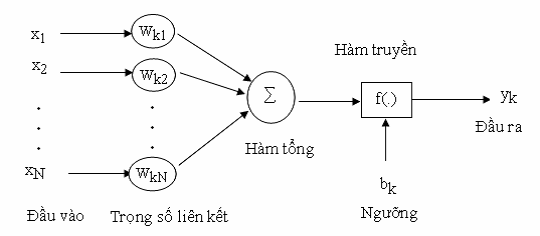
\includegraphics[scale=1.0]{Appendix1/nerualnhantao}
    \else
      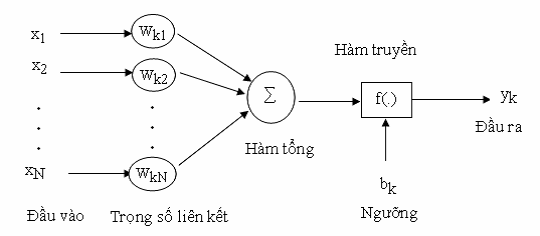
\includegraphics[scale=1.0]{Appendix1/nerualnhantao}
    \fi
    \caption{Cấu trúc nơron nhân tạo}
    \label{neuralnhantao}
  \end{center}
\end{figure}

Các thành phần cơ bản của một nơron nhân tạo bao gồm: 
\begin{itemize}
\item \textbf{Tập các đầu vào}: Là các tín hiệu vào (\textit{input signals}) của nơron, các tín hiệu này thường được đưa vào dưới dạng một vector N chiều. 
\item \textbf{Tập các liên kết}: Mỗi liên kết được thể hiện bởi một trọng số (gọi là trọng số liên kết – S\textit{ynaptic weight}). Trọng số liên kết giữa tín hiệu vào thứ j với nơron k thường được kí hiệu là wkj. Thông thường, các trọng số này được khởi tạo một cách ngẫu nhiên ở thời điểm khởi tạo mạng và được cập nhật liên tục trong quá trình học mạng. 
\item \textbf{Bộ tổng} (\textit{Summing function}): Thường dùng để tính tổng của tích các đầu vào với trọng số liên kết của nó. 
\item \textbf{Ngưỡng} (còn gọi là một độ lệch - \textit{bias}): Ngưỡng này thường được đưa vào như một thành phần của hàm truyền. 
\item \textbf{Hàm truyền} (\textit{Transfer function}) : Hàm này được dùng để giới hạn phạm vi đầu ra của mỗi nơron. Nó nhận đầu vào là kết quả của hàm tổng và ngưỡng đã cho. Thông thường, phạm vi đầu ra của mỗi nơron được giới hạn trong đoạn [0,1] hoặc [-1, 1]. Các hàm truyền rất đa dạng, có thể là các hàm tuyến tính hoặc phi tuyến. Việc lựa chọn hàm truyền nào là tuỳ thuộc vào từng bài toán và kinh nghiệm của người thiết kế mạng.
\item \textbf{Đầu ra}: Là tín hiệu đầu ra của một nơron, với mỗi nơron sẽ có tối đa là một đầu ra. 
\end{itemize}

\subsection{Kiến trúc mạng nơron}
Người ta chia mạng nơron làm hai kiến trúc: 
\begin{itemize}

\item \textbf{Kiến trúc truyền thẳng} (\textit{feedforward architechture}): là kiểu kiến trúc mạng không có các kết nối ngược trở lại từ các nơron đầu ra về các nơron đầu vào; mạng không lưu lại các giá trị output trước và các trạng thái kích hoạt của nơron. Các mạng nơron truyền thẳng cho phép tín hiệu di chuyển theo một đường duy nhất; từ đầu vào tới đầu ra, đầu ra của một tầng bất kì sẽ không ảnh hưởng tới tầng đó.
\item \textbf{Kiến trúc phản hồi} (\textit{Feedback architecture}): là kiểu kiến trúc mạng có các kết nối từ nơron đầu ra tới nơron đầu vào. Mạng lưu lại các trạng thái trước đó, và trạng thái tiếp theo không chỉ phụ thuộc vào các tín hiệu đầu vào mà còn phụ thuộc vào các trạng thái trước đó của mạng.
\end{itemize}